 
\chapter{Progetto}

\section{Specifica dell’architettura}
 Il sistema è accessibile tramite browser, in particolare sfrutta un'architettura di tipo \emph{client-server}, il client è il dispositivo da cui accede l’utente, che comunicano con Web Browser  tramite protocollo \emph{HTTPS} in modo da garantire uno scambio dei dati sicuro tra le due estremità. Il sistema principale si interfaccia (tramite \emph{HTTPS} e \emph{TCP/IP}) con gli altri sistemi che sono: il \textbf{Database delle Aule} tramite un \emph{DBMS} che viene interrogato all’occorrenza, il \textbf{Database delle prenotazioni} contenente tutte le prenotazioni, il sistema \textbf{Infostud} tramite il quale verifica le credenziali d’accesso e richiede informazioni  necessarie sullo studente che sono contenute nel  \textbf{Database degli studenti}. Infine è presente un \textbf{server di posta elettronica} (lo stesso che usa Infostud) per l’invio delle e-mail. La figura ~\ref{figura: digramma architetturale} mostra un grafico esplicativo del design architetturale.
 
 \begin{figure}[H]
\begin{center}	
  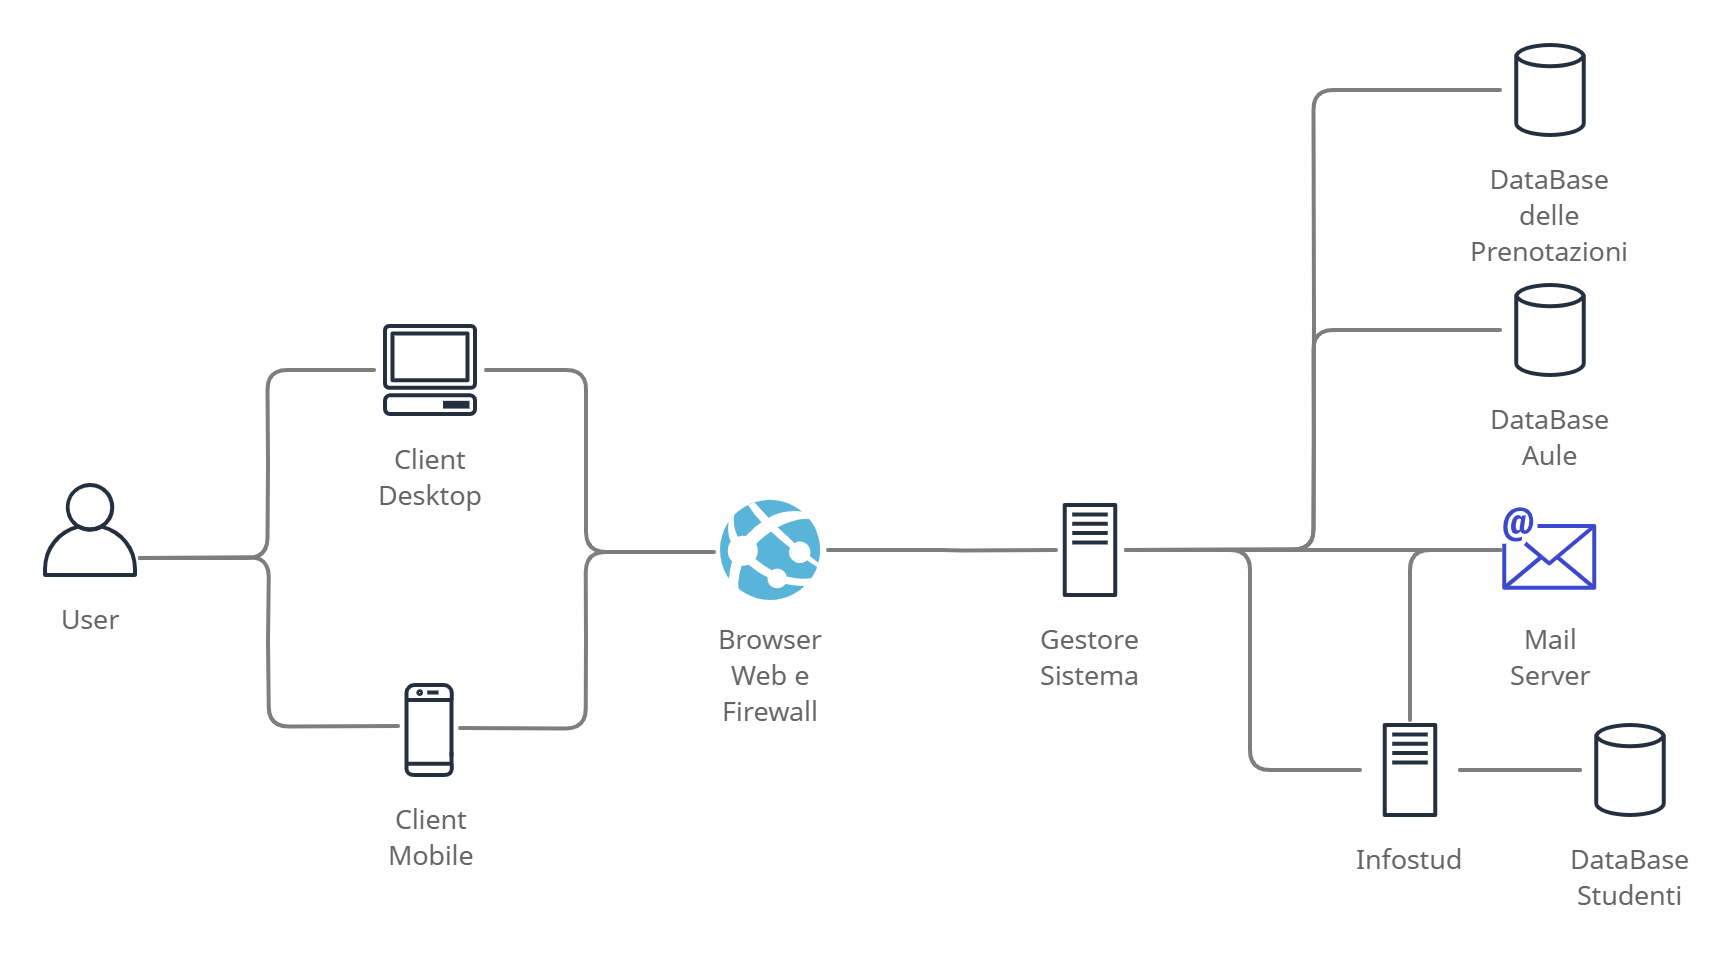
\includegraphics[width=1 \textwidth]{Figure/diagramma architetturale.jpg}
    \caption{Diagramma dell’architettura.}\label{figura: digramma architetturale}
\end{center}
\end{figure}



\section {Classi di progetto}

 
La classe \textbf{Studente} ha solo il metodo per ottenere i dati,  (es. matricola o indirizzo mail) \textbf{GetInfo()}, non ha altri metodi per aggiornare le informaizoni poichè queste vengopno modifciate all’interno del sistema Infostud.\\

\noindent La classe \textbf{Aula} ha diversi metodi per la gestione, in particolare: \textbf{SetState()} che permette di aggiornare lo stato dell’aula (se non dovesse essere disponibile), \textbf{GetState()} permette di ottenere lo stato dell’aula, \textbf{GetCapacity()}, la capienza Covid dell’aula e \textbf{SetCapacity()} imposta la capienza dell’aula (se si ha la necessità di dover ampliare o ridurre la capienza), i metodi \textbf{GetInfo()} e \textbf{SetInfo()} servono rispettivamente per ottenere e aggioranre le informazioni inerenti all’aula.\\
 
 
\noindent La classe \textbf{Prenotazione}, usa il metodo \textbf{CreatePrenotazione()} per creare una prenotazione riferita ad uno studente e ad un’aula, \textbf{CreateRicevuta()} crea la ricevuta a partire dalla prenotazione create, ricevuta da mandare per mail tramite il metodo \textbf{SendMail()}, \textbf{SendAllert()} serve per inviare un messaggio d’errore in caso l’utente non sia abilitato a prenotarsi, oppure nel caso in cui si prova a fare una prenotazione multipla dell’aula nella stessa fascia oraria o nel caso ci sia un errore nell’inserimento dei dati. \\
 

\noindent La classe \textbf{GestsiciPrenotazioni} è in dipendenza di tipo \emph{<<use>>} alla classe \textbf{Prenotazioni} poiché essa necessita della seconda per operare. La classe ha i seguenti metodi: \textbf{DeletePrenotazione()} per cancellare una determinata prenotazione,  \textbf{ViewPrenotazione()} per vedere le prenotazioni effettuate, \textbf{ViewStatePrenotazione()} per ottenere lo stato (effettuata, cancellata o in attesa) di una determinata prenotazione, \textbf{DowloadRicevuta()} per scaricare la ricevuta di una prenotazione e  \textbf{ViewRicevuta()} per visalizzare la ricevuta. \\


\noindent La classe \textbf{Coda} si occupa di gestire le code per le prenotazioni delle aule, con il metodo \textbf{AddToQueue()} aggiunge lo studente alla coda nel caso in cui l’aula sia piena, \textbf{RemoveFromQueue()} rimuove uno studente dalla coda (aggiornandola) nel caso in cui abbia cancellato la prenotazione rtiferita all’aula, oppure nel caso in cui il primo studente della coda  viene aggiunto alle prenotazioni effettuate (per scorrimento), \textbf{UpdateStatoPrenotazione()} aggiorna lo stato di una prenotazione quando si esce dalla coda (es. effettuata o cancellata), infine con \textbf{SendMail()} viene inviata una mail di notfica nel caso in cui si verifichi un cambiamento all’interno della coda.


\noindent La figura ~\ref{figura: digramma delle classi} riporta quanto detto ma sottoforma di diagramma delle classi.\\

 \begin{figure}[htp]
\begin{center}
  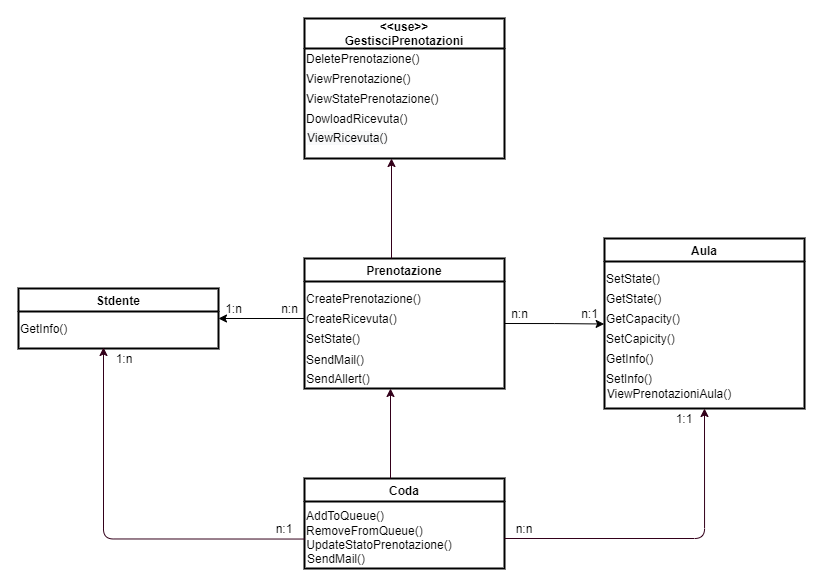
\includegraphics[width=1 \textwidth]{Figure/class diagram.png}
    \caption{Diagramma delle classi.}\label{figura: digramma delle classi}
\end{center}
\end{figure}

Le molteplicità tra la classe \textbf{Studente} e \textbf{Prenotazione}: \emph{(1:n)} indica che ad uno studente corrispondono n prenotazioni, \emph{(n:n)} che ad n prenotazioni corrispondono n studenti; quella tra le classi \textbf{Prenotazione} e \textbf{Aula} indicano: \emph{(n:1)} che ad un’aula corrispondono n prenotazioni, ma \emph{(n:n)} che ad n prenotazioni corrispondono n aule.\\
Le molteplicità tra la classe \textbf{Coda} e la classe \textbf{Studente} rappresenta il fatto che uno studente può trovarsi in n code \emph{(1:n)} e che in una coda possono esserci n studenti \emph{(n:1)}. Le molteplicità tra le classi \textbf{Coda} ed \textbf{Aula} indicanno che ad un’aula corrisponde una ed una sola coda \emph{(1:1)} mentre ad n code corrispondono n aule \emph{(n:n)}.


\section{Sequence diagrams}

In questa sezione ci interessa descrivere le azioni svolte per un determinato caso d’uso, raffigurandole tramite i diagrammi di sequenza.


 \begin{figure}[H]
\begin{center}
  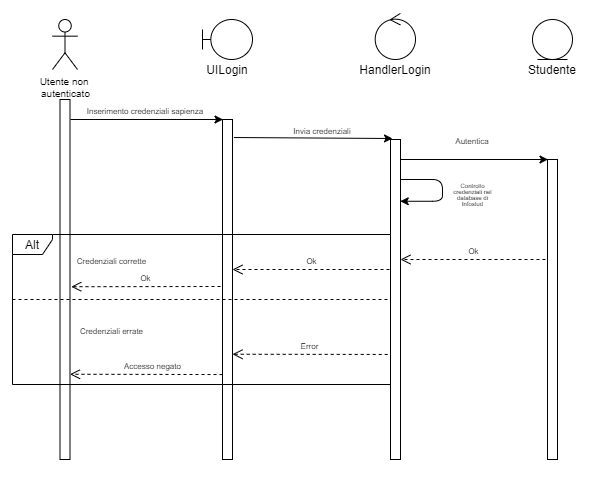
\includegraphics[width=1 \textwidth]{Figure/sequence login.png}
    \caption{Diagramma di sequenza per il login.}\label{figura: login}
\end{center}
\end{figure}


 \begin{figure}[H]
\begin{center}
  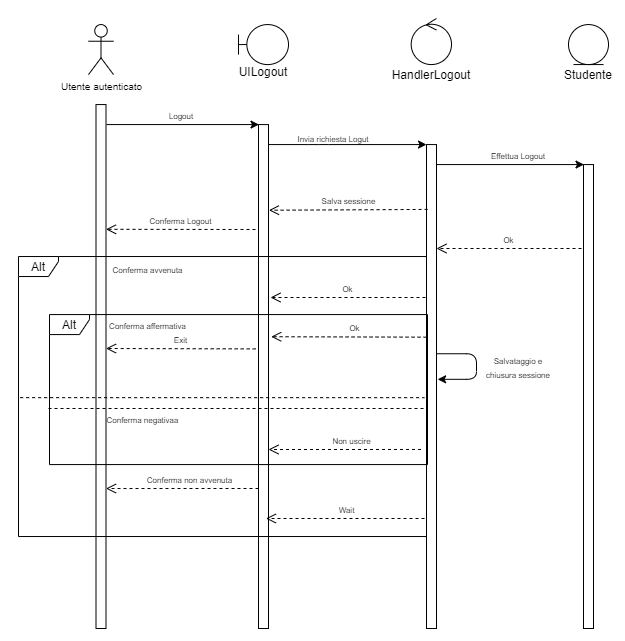
\includegraphics[width=1 \textwidth]{Figure/sequence logout.png}
    \caption{Diagramma di sequenza per il logout.}\label{figura: logout}
\end{center}
\end{figure}

 \begin{figure}[H]
\begin{center}
  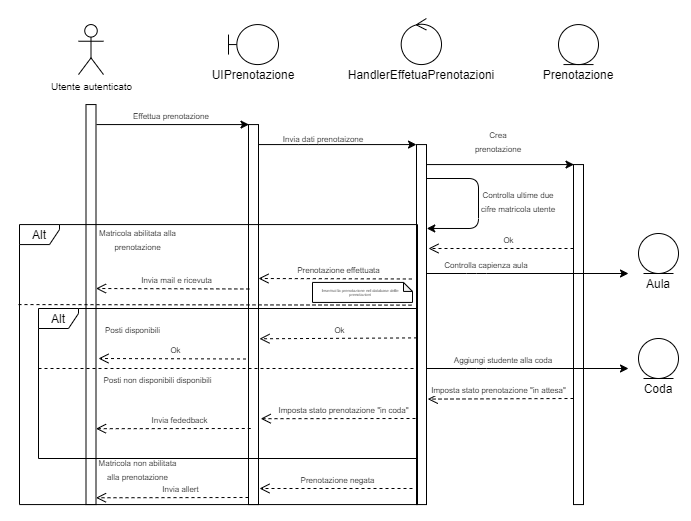
\includegraphics[width=1 \textwidth]{Figure/sequence prenotazione.png}
    \caption{Diagramma di sequenza che mostra come effettuare la prenotazione.}\label{figura: effettua}
\end{center}
\end{figure}


 \begin{figure}[H]
\begin{center}
  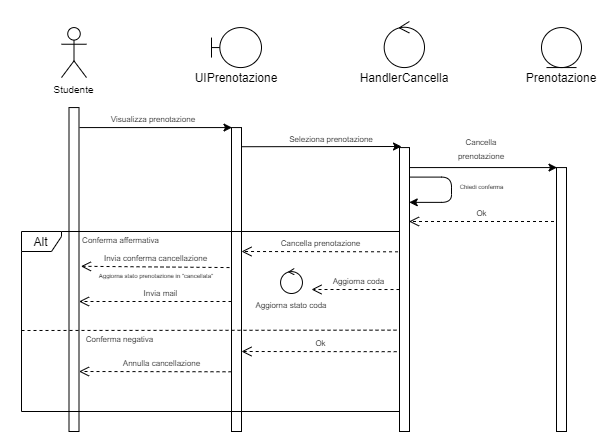
\includegraphics[width=1 \textwidth]{Figure/sequence cancella.png}
    \caption{Diagramma di sequenza cancellazione prenotazione.}\label{figura: cancella}
\end{center}
\end{figure}

\begin{figure}[H]
\begin{center}
  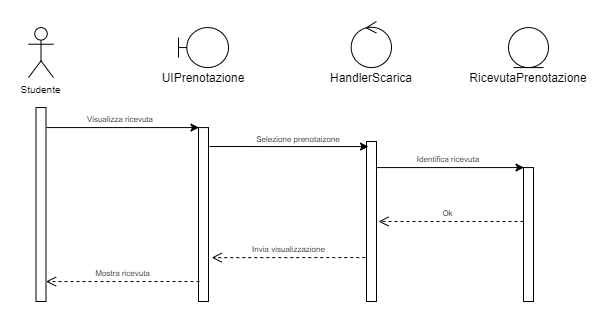
\includegraphics[width=1 \textwidth]{Figure/sequence visualizza.png}
    \caption{Diagramma di sequenza visualizzazione prenotazione.}\label{figura: visualizza}
\end{center}
\end{figure}


\begin{figure}[H]
\begin{center}
  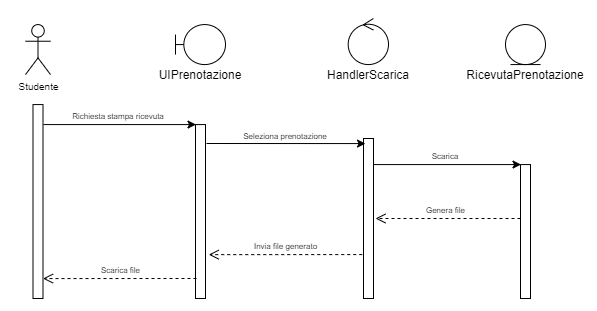
\includegraphics[width=1 \textwidth]{Figure/sequence scarica.png}
    \caption{Diagramma di sequenza perlo scaricamento della ricevuta in PDF.}\label{figura: scarica}
\end{center}
\end{figure}


\begin{figure}[H]
\begin{center}
  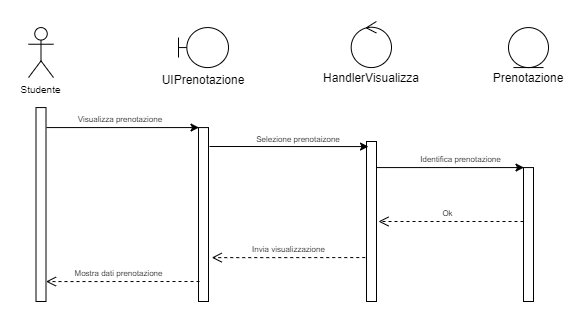
\includegraphics[width=1 \textwidth]{Figure/sequence visualizza ricevuta.png}
    \caption{Diagramma di sequenza visualizzazione ricevuta.}\label{figura: visualizza ricevuta}
\end{center}
\end{figure}



\section{Cicli di vita delle classi}
Per identificare i cicli di vita delle classi ci si deve riferire agli oggetti che possono cambiare stato a seguito di eventi, in particolare in questo caso si farà riferimento solo alla classe  \textbf{Prenotazione} (figura ~\ref{figura: ciclo prenotazione}) e alla classe \textbf{Aula} (figura ~\ref{figura: digramma delle classi}).


\begin{figure}[H]
\begin{center}
  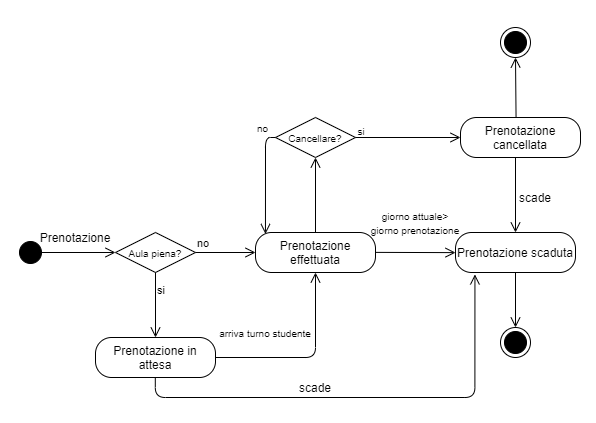
\includegraphics[width=1 \textwidth]{Figure/ciclo classe prenotazione.png}
    \caption{Ciclo di vita della classe \textbf{Prenotazione}}  \label{figura: ciclo prenotazione}
\end{center}
\end{figure}


\begin{figure}[H]
\begin{center}
  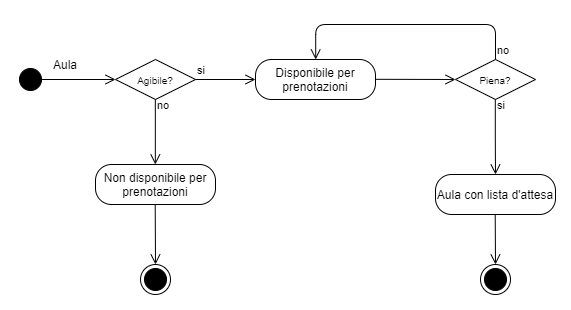
\includegraphics[width=1 \textwidth]{Figure/ciclo classe aula.png}
    \caption{Ciclo di vita della classe \textbf{Aula}}\label{figura: ciclo aula}
\end{center}
\end{figure}
